{\centering{\section*{\textit{K-nearest neighbor}}%
\label{sec:K-nearest neighbor}
}}
\subsection*{基本思路}%
\label{sub:基本思路}
找到与新输入的待预测样本最临近的$K$ 个样本,判断这$K$ 个样本中绝大多数的所属类别作为分类结果输出

条件:已经具有较大的样本量
\begin{center}
    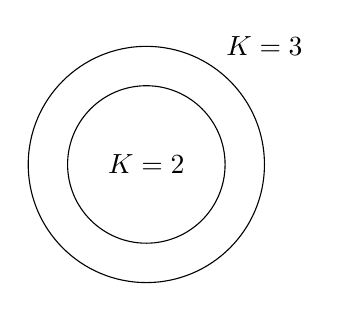
\begin{tikzpicture}
        \draw [] (0,0) circle [radius=1] node at(0,0) {$K=2$};
        \draw [] (0,0) circle [radius=1.5] node at(1.5,1.5) {$K=3$};
    \end{tikzpicture}
\end{center}
\begin{notation}
    KNN算法的基本要素:距离度量、$K$ 值、分类决策规则
\end{notation}
\subsection*{距离度量}%
\label{sub:距离度量}
\begin{notation}
    KNN算法能够分类:特征空间内的样本点之间的距离能够反映样本特征的相似程度
\end{notation}
设有两个样本点$\bm{x}_{i},\bm{x}_{j}$ ,以$n$ 维向量空间作为特征空间,将这两个点表示为:
\[
    \bm{x}_i,\bm{x}_{j}\in \bm{X}
.\]
\[
    \bm{x}_i=\left( x_{i}^{1},x_{i}^2,\ldots,x_{i}^{n} \right)^{T}
.\] 
\[
    \bm{x}_j=\left( x_{j}^1.x_{j}^2,\ldots,x_{j}^{n} \right) ^{T}
.\] 

特征点之间的距离定义为:
\[
    L_p\left( \bm{x}_i,\bm{x}_j \right) =\left( \sum_{l=1}^{n} \left| x_{i}^{l}-x_{j}^{l} \right|^{p}  \right) ^{\frac{1}{p}}
.\] 
\begin{eg}
    代入$p=2$ ,易得$L_2\left( \bm{x}_i,\bm{x}_j \right) $为平面上两点间的距离公式,该距离又称为欧氏距离:
    \[
        L_2\left( \bm{x}_i,\bm{x}_j \right) =\sqrt{\left( x_{i_1}-x_{j_1} \right) ^2+\left( x_{i_2}-x_{j_2} \right) ^2} 
    .\] 
    \begin{center}
        \begin{tikzpicture}
            \draw [] (-1,1) circle [radius=2pt] node at(-1.5,1.5) {$A$};
            \draw [] (1,-1) circle [radius=2pt] node at(1.5,-1.5) {$B$};
            \draw [] (-1,1)--(1,-1);
            \node at(-1.5,-1.5) {$L_2\left( A,B \right) =2\sqrt{2} $};
        \end{tikzpicture}
    \end{center}

    代入$p=1$ :$L_1\left( x_{i},x_{j} \right) $ 称为曼哈顿距离:
    \begin{center}
        \begin{tikzpicture}
            \draw [] (-1,1) circle [radius=2pt] node at(-1.5,1.5) {$A$};
            \draw [] (1,-1) circle [radius=2pt] node at(1.5,-1.5) {$B$};
            \draw [dashed] (-1,1)--(1,-1);
            \draw [] (-1,1)--(-1,0)--(0,0)--(0,-1)--(1,-1);
            \draw [] (-1,1)--(1,1)--(1,-1);
            \node at(-1.5,-1.5) {$L_1\left( A,B \right) =4$};
        \end{tikzpicture}
    \end{center}
\end{eg}
\subsection*{\textit{K}值的选择}%
\label{sub:K值的选择}
使用交叉验证方法确定最合适的$K$ 值
